% Options for packages loaded elsewhere
\PassOptionsToPackage{unicode}{hyperref}
\PassOptionsToPackage{hyphens}{url}
\PassOptionsToPackage{dvipsnames,svgnames,x11names}{xcolor}
%
\documentclass[
  11pt,
]{article}
\usepackage{amsmath,amssymb}
\usepackage{iftex}
\ifPDFTeX
  \usepackage[T1]{fontenc}
  \usepackage[utf8]{inputenc}
  \usepackage{textcomp} % provide euro and other symbols
\else % if luatex or xetex
  \usepackage{unicode-math} % this also loads fontspec
  \defaultfontfeatures{Scale=MatchLowercase}
  \defaultfontfeatures[\rmfamily]{Ligatures=TeX,Scale=1}
\fi
\usepackage{lmodern}
\ifPDFTeX\else
  % xetex/luatex font selection
  \setmainfont[]{Latin Modern Roman}
  \setmonofont[]{Latin Modern Mono}
\fi
% Use upquote if available, for straight quotes in verbatim environments
\IfFileExists{upquote.sty}{\usepackage{upquote}}{}
\IfFileExists{microtype.sty}{% use microtype if available
  \usepackage[]{microtype}
  \UseMicrotypeSet[protrusion]{basicmath} % disable protrusion for tt fonts
}{}
\makeatletter
\@ifundefined{KOMAClassName}{% if non-KOMA class
  \IfFileExists{parskip.sty}{%
    \usepackage{parskip}
  }{% else
    \setlength{\parindent}{0pt}
    \setlength{\parskip}{6pt plus 2pt minus 1pt}}
}{% if KOMA class
  \KOMAoptions{parskip=half}}
\makeatother
\usepackage{xcolor}
\usepackage[margin=2.5cm]{geometry}
\usepackage{color}
\usepackage{fancyvrb}
\newcommand{\VerbBar}{|}
\newcommand{\VERB}{\Verb[commandchars=\\\{\}]}
\DefineVerbatimEnvironment{Highlighting}{Verbatim}{commandchars=\\\{\}}
% Add ',fontsize=\small' for more characters per line
\newenvironment{Shaded}{}{}
\newcommand{\AlertTok}[1]{\textcolor[rgb]{1.00,0.00,0.00}{\textbf{#1}}}
\newcommand{\AnnotationTok}[1]{\textcolor[rgb]{0.38,0.63,0.69}{\textbf{\textit{#1}}}}
\newcommand{\AttributeTok}[1]{\textcolor[rgb]{0.49,0.56,0.16}{#1}}
\newcommand{\BaseNTok}[1]{\textcolor[rgb]{0.25,0.63,0.44}{#1}}
\newcommand{\BuiltInTok}[1]{\textcolor[rgb]{0.00,0.50,0.00}{#1}}
\newcommand{\CharTok}[1]{\textcolor[rgb]{0.25,0.44,0.63}{#1}}
\newcommand{\CommentTok}[1]{\textcolor[rgb]{0.38,0.63,0.69}{\textit{#1}}}
\newcommand{\CommentVarTok}[1]{\textcolor[rgb]{0.38,0.63,0.69}{\textbf{\textit{#1}}}}
\newcommand{\ConstantTok}[1]{\textcolor[rgb]{0.53,0.00,0.00}{#1}}
\newcommand{\ControlFlowTok}[1]{\textcolor[rgb]{0.00,0.44,0.13}{\textbf{#1}}}
\newcommand{\DataTypeTok}[1]{\textcolor[rgb]{0.56,0.13,0.00}{#1}}
\newcommand{\DecValTok}[1]{\textcolor[rgb]{0.25,0.63,0.44}{#1}}
\newcommand{\DocumentationTok}[1]{\textcolor[rgb]{0.73,0.13,0.13}{\textit{#1}}}
\newcommand{\ErrorTok}[1]{\textcolor[rgb]{1.00,0.00,0.00}{\textbf{#1}}}
\newcommand{\ExtensionTok}[1]{#1}
\newcommand{\FloatTok}[1]{\textcolor[rgb]{0.25,0.63,0.44}{#1}}
\newcommand{\FunctionTok}[1]{\textcolor[rgb]{0.02,0.16,0.49}{#1}}
\newcommand{\ImportTok}[1]{\textcolor[rgb]{0.00,0.50,0.00}{\textbf{#1}}}
\newcommand{\InformationTok}[1]{\textcolor[rgb]{0.38,0.63,0.69}{\textbf{\textit{#1}}}}
\newcommand{\KeywordTok}[1]{\textcolor[rgb]{0.00,0.44,0.13}{\textbf{#1}}}
\newcommand{\NormalTok}[1]{#1}
\newcommand{\OperatorTok}[1]{\textcolor[rgb]{0.40,0.40,0.40}{#1}}
\newcommand{\OtherTok}[1]{\textcolor[rgb]{0.00,0.44,0.13}{#1}}
\newcommand{\PreprocessorTok}[1]{\textcolor[rgb]{0.74,0.48,0.00}{#1}}
\newcommand{\RegionMarkerTok}[1]{#1}
\newcommand{\SpecialCharTok}[1]{\textcolor[rgb]{0.25,0.44,0.63}{#1}}
\newcommand{\SpecialStringTok}[1]{\textcolor[rgb]{0.73,0.40,0.53}{#1}}
\newcommand{\StringTok}[1]{\textcolor[rgb]{0.25,0.44,0.63}{#1}}
\newcommand{\VariableTok}[1]{\textcolor[rgb]{0.10,0.09,0.49}{#1}}
\newcommand{\VerbatimStringTok}[1]{\textcolor[rgb]{0.25,0.44,0.63}{#1}}
\newcommand{\WarningTok}[1]{\textcolor[rgb]{0.38,0.63,0.69}{\textbf{\textit{#1}}}}
\usepackage{longtable,booktabs,array}
\usepackage{calc} % for calculating minipage widths
% Correct order of tables after \paragraph or \subparagraph
\usepackage{etoolbox}
\makeatletter
\patchcmd\longtable{\par}{\if@noskipsec\mbox{}\fi\par}{}{}
\makeatother
% Allow footnotes in longtable head/foot
\IfFileExists{footnotehyper.sty}{\usepackage{footnotehyper}}{\usepackage{footnote}}
\makesavenoteenv{longtable}
\usepackage{graphicx}
\makeatletter
\def\maxwidth{\ifdim\Gin@nat@width>\linewidth\linewidth\else\Gin@nat@width\fi}
\def\maxheight{\ifdim\Gin@nat@height>\textheight\textheight\else\Gin@nat@height\fi}
\makeatother
% Scale images if necessary, so that they will not overflow the page
% margins by default, and it is still possible to overwrite the defaults
% using explicit options in \includegraphics[width, height, ...]{}
\setkeys{Gin}{width=\maxwidth,height=\maxheight,keepaspectratio}
% Set default figure placement to htbp
\makeatletter
\def\fps@figure{htbp}
\makeatother
\setlength{\emergencystretch}{3em} % prevent overfull lines
\providecommand{\tightlist}{%
  \setlength{\itemsep}{0pt}\setlength{\parskip}{0pt}}
\setcounter{secnumdepth}{-\maxdimen} % remove section numbering
\ifLuaTeX
\usepackage[bidi=basic]{babel}
\else
\usepackage[bidi=default]{babel}
\fi
\babelprovide[main,import]{polish}
\ifPDFTeX
\else
\babelfont{rm}[]{Latin Modern Roman}
\fi
% get rid of language-specific shorthands (see #6817):
\let\LanguageShortHands\languageshorthands
\def\languageshorthands#1{}
% Ładne, czytelne tabele: booktabs + zebra-striping + pełna szerokość strony.
\usepackage{etoolbox}
\usepackage{graphicx}
\usepackage{booktabs}
\usepackage{tabularx}
\usepackage[table]{xcolor}
\usepackage{array}

% Kolory zebry (delikatny szary co drugi wiersz).
\definecolor{zebragray}{gray}{0.93}

% Typy kolumn dla tabularx: L = lewa (rozciągliwa), R = prawa (rozciągliwa).
\newcolumntype{L}{>{\raggedright\arraybackslash}X}
\newcolumntype{R}{>{\raggedleft\arraybackslash}X}

% Gęste tabele metryk: nieco mniejsza czcionka, luźniejsze wiersze.
\setlength{\tabcolsep}{5pt}
\renewcommand{\arraystretch}{1.25}

% Obrazy nie szersze niż tekst.
\setkeys{Gin}{width=\linewidth,keepaspectratio}
\ifLuaTeX
  \usepackage{selnolig}  % disable illegal ligatures
\fi
\IfFileExists{bookmark.sty}{\usepackage{bookmark}}{\usepackage{hyperref}}
\IfFileExists{xurl.sty}{\usepackage{xurl}}{} % add URL line breaks if available
\urlstyle{same}
\hypersetup{
  pdftitle={Detekcja samolotów na zdjęciach satelitarnych pod przesunięciem domeny synthetic-to-real},
  pdfauthor={Jakub Paszke; Miłosz Rolewski},
  pdflang={pl},
  colorlinks=true,
  linkcolor={blue},
  filecolor={Maroon},
  citecolor={Blue},
  urlcolor={blue},
  pdfcreator={LaTeX via pandoc}}

\title{Detekcja samolotów na zdjęciach satelitarnych pod przesunięciem
domeny synthetic-to-real}
\usepackage{etoolbox}
\makeatletter
\providecommand{\subtitle}[1]{% add subtitle to \maketitle
  \apptocmd{\@title}{\par {\large #1 \par}}{}{}
}
\makeatother
\subtitle{Projekt 4 --- Deep Learning / Computer Vision}
\author{Jakub Paszke \and Miłosz Rolewski}
\date{Czerwiec 2026}

\begin{document}
\maketitle

{
\hypersetup{linkcolor=}
\setcounter{tocdepth}{2}
\tableofcontents
}
\hypertarget{abstrakt}{%
\subsection{Abstrakt}\label{abstrakt}}

Projekt bada lukę domenową między syntetycznymi i rzeczywistymi
zdjęciami satelitarnymi w zadaniu detekcji samolotów na zbiorze
RarePlanes. Głównym modelem eksperymentalnym był YOLOv10n trenowany w
formacie YOLO po konwersji adnotacji COCO, a jako metryki porównawcze
przyjęto ewaluację COCO na rzeczywistym holdoucie testowym. Punkt
odniesienia trenowany i testowany na danych realnych osiągnął
\texttt{AP@.5=0.9737} oraz \texttt{AP@{[}.5:.95{]}=0.8073}. Naiwny
transfer z pełnej syntetyki 45k na realny test był dużo słabszy:
\texttt{AP@.5=0.4525}, \texttt{AP@{[}.5:.95{]}=0.2683}.

Przetestowano cztery rodziny interwencji: fotometrię HSV, degradację
częstotliwościową, mixed training z domieszką realnych obrazów oraz
zmianę rozdzielczości wejścia. Najsilniejszy wynik dał eksperyment C:
dodanie 25\% dostępnego realnego train/val do 10k syntetyków, co
odpowiadało około 11\% realnych obrazów w zbiorze treningowym, podniosło
wynik do \texttt{AP@.5=0.9466} i \texttt{AP@{[}.5:.95{]}=0.7120}. Model
finalny 45k połączył decyzje B2+C+D+A1: szum \texttt{noise\_sigma=8.0},
\texttt{real\_frac=0.25}, \texttt{imgsz=320} i łagodne HSV
\texttt{0.015/0.4/0.3}. Osiągnął \texttt{AP@.5=0.9031} oraz
\texttt{AP@{[}.5:.95{]}=0.6332}, czyli bardzo poprawił czysty baseline
synthetic 45k, ale nie przebił C 25\% na 10k. Główny wniosek jest więc
praktyczny: realne próbki działają jak kotwica domenowa silniej niż sama
ekspansja syntetyki, a efekty dobrych decyzji nie sumują się liniowo.

\hypertarget{pytanie-badawcze-i-hipotezy}{%
\subsection{Pytanie badawcze i
hipotezy}\label{pytanie-badawcze-i-hipotezy}}

Dane syntetyczne są atrakcyjne w detekcji obiektów, bo pozwalają
generować duże zbiory z pełnymi adnotacjami bez kosztownego ręcznego
etykietowania. Ich problemem jest jednak luka domenowa: model dobrze
dopasowany do renderów może gwałtownie tracić jakość na obrazach
rzeczywistych. RarePlanes jest dobrym przypadkiem testowym, bo zawiera
zarówno dane realne, jak i syntetyczne dla tego samego zadania: detekcji
samolotów w kaflach satelitarnych.

Pytanie badawcze:

\begin{Shaded}
\begin{Highlighting}[]
\NormalTok{Jak skutecznie zmniejszyć spadek jakości detektora trenowanego na syntetycznych}
\NormalTok{zdjęciach RarePlanes po przeniesieniu na rzeczywiste zdjęcia satelitarne?}
\end{Highlighting}
\end{Shaded}

Hipotezy projektu:

\begingroup
\rowcolors{2}{zebragray}{white}
\noindent\resizebox{\linewidth}{!}{%
\begin{tabular}{lll}
\toprule
Hipoteza & Treść & Eksperyment \\
\midrule

\bottomrule

HA & Dopasowanie fotometrii i augmentacja HSV zmniejszą różnice
kolorystyczne synthetic-real. & A \\
HB & Szum i degradacje częstotliwościowe upodobnią synthetic do realnych
zdjęć satelitarnych. & B \\
HC & Nawet niewielka liczba realnych próbek mocno poprawi transfer. &
C \\
HD & Zmiana skali wejścia pomoże wykrywaniu małych realnych obiektów. &
D \\
HArch & Architektura wpływa na odporność modelu na domain shift. &
porównanie architektur \\
\end{tabular}%
}
\endgroup


Wyniki odwróciły część intuicji. Szczególnie hipoteza HD została
potwierdzona w kierunku przeciwnym do pierwotnej intuicji: nie większa,
lecz mniejsza rozdzielczość \texttt{imgsz=320} poprawiła transfer.

\hypertarget{przeglux105d-literatury}{%
\subsection{Przegląd literatury}\label{przeglux105d-literatury}}

Luka domenowa między danymi syntetycznymi a rzeczywistymi jest jednym z
centralnych problemów uczenia z renderów. Klasyczne podejście
\emph{domain randomization} (Tobin i in., IROS 2017, arXiv:1703.06907)
zakłada, że losowanie tekstur, oświetlenia i tła w symulacji zmusza
model do uczenia się cech niezmienniczych względem domeny --- przy
dostatecznej zmienności symulacji rzeczywistość staje się dla modelu
"kolejnym wariantem". Nasze eksperymenty A i B mieszczą się w tej
rodzinie: HSV i degradacja częstotliwościowa to próby zasypania
mierzalnych różnic fotometryczno-spektralnych między domenami. Nasze
wyniki pokazują jednak, że taka korekta na poziomie obrazu domyka lukę
tylko marginalnie (A1: \texttt{AP@.5=0.4591}, B2: \texttt{0.4897} wobec
baseline \texttt{0.4525}).

Drugą rodziną metod jest adaptacja przez domieszkę danych docelowych.
Prace o \emph{few-shot} i mieszanym treningu pokazują, że nawet
niewielki udział realnych próbek silnie kotwiczy reprezentację w domenie
docelowej --- co w naszym projekcie potwierdza eksperyment C i czyni go
najsilniejszą dźwignią (już 1\% realnego splitu podnosi \texttt{AP@.5} z
\texttt{0.4525} do \texttt{0.6666}). Jest to spójne z szerszą obserwacją
z nurtu \emph{data-centric}, że dobór danych treningowych bywa
ważniejszy niż architektura: w naszych pomiarach zmiana składu danych
dała \texttt{+0.49\ AP@.5}, a zmiana architektury jedynie
\texttt{+0.008}.

Zbiór \textbf{RarePlanes} (Shermeyer i in., 2020, arXiv:2006.02963)
został zaprojektowany właśnie do badania tej luki: dostarcza dane
rzeczywiste (253 sceny Maxar WorldView-3, \textasciitilde14,7 tys.
ręcznie oznaczonych samolotów) oraz syntetyczne (\textasciitilde50 tys.
obrazów z platformy AI.Reverie, \textasciitilde600 tys. adnotacji), z
bogatą semantyką ról i atrybutów. Oryginalna praca pokazała, że dodanie
syntetyki do realnego treningu poprawia detekcję; nasz projekt zadaje
pytanie odwrotne --- jak daleko można zajść \emph{zaczynając} od
syntetyki i dokładając jak najmniej realnych danych.

Po stronie architektur porównujemy jednostopniowe detektory CNN z
rodziny YOLO (YOLOv10, Wang i in., NeurIPS 2024, arXiv:2405.14458) z
detektorami transformerowymi typu DETR w wariancie czasu rzeczywistego
(RT-DETR, Lv i in., 2023, arXiv:2304.08069). Co istotne dla naszej
obserwacji, \emph{obie} te architektury są end-to-end i rezygnują z NMS
--- YOLOv10 przez spójne podwójne przypisania w treningu, RT-DETR przez
paradygmat predykcji zbioru z dopasowaniem węgierskim. Pozwala to wprost
zbadać, czy brak NMS pomaga, czy szkodzi pod przesunięciem domeny: w
naszych wynikach oba modele RT-DETR zwracają maksymalne 300 detekcji na
obraz na realnym teście, co sugeruje, że mechanizm bez progu/NMS gorzej
kalibruje się na obcej domenie. Do interpretowalności używamy EigenCAM
(Muhammad i Yeasin, IJCNN 2020, arXiv:2008.00299) --- wariantu opartego
na głównych składowych aktywacji, który nie wymaga gradientu względem
klasy, a więc lepiej pasuje do detektorów end-to-end niż klasyczny
Grad-CAM.

\hypertarget{dane-rareplanes-i-licencja}{%
\subsection{Dane RarePlanes i
licencja}\label{dane-rareplanes-i-licencja}}

Projekt korzysta ze zbioru RarePlanes, Shermeyer et al., 2020,
udostępnionego na licencji Creative Commons Attribution-ShareAlike 4.0
International. W repozytorium nie redystrybuowano obrazów. Dane są
pobierane i przetwarzane skryptami, a w gicie pozostają kod, notatki,
lekkie wyniki oraz figury.

Użyty wariant obrazów realnych to \texttt{PS-RGB\_tiled}: kafle RGB
porównywalne z obrazami syntetycznymi. Warianty MS/PAN pominięto, bo
mają inne kanały i nie byłyby bezpośrednio porównywalne z syntetycznym
RGB. Zadanie sprowadzono do jednej klasy \texttt{aircraft}, aby mierzyć
lokalizację samolotów bez dodatkowego problemu klasyfikacji ról.

\begingroup
\rowcolors{2}{zebragray}{white}
\begin{tabularx}{\linewidth}{LRRR}
\toprule
Zbiór & Obrazy & Instancje & Instancje/obraz \\
\midrule

\bottomrule

real train & 5 815 & 18 393 & 3.16 \\
real test & 2 710 & 6 812 & 2.51 \\
synthetic train & 45 000 & 566 143 & 12.58 \\
synthetic test & 5 000 & 62 841 & 12.57 \\
\end{tabularx}
\endgroup


\hypertarget{analiza-domain-shift}{%
\subsection{Analiza domain shift}\label{analiza-domain-shift}}

\hypertarget{rozmiar-obiektuxf3w-i-gux119stoux15bux107-scen}{%
\subsubsection{Rozmiar obiektów i gęstość
scen}\label{rozmiar-obiektuxf3w-i-gux119stoux15bux107-scen}}

Najsilniejszy shift adnotacyjny dotyczy rozmiaru samolotów i gęstości
scen. Dane syntetyczne mają znacznie więcej obiektów na obraz oraz dużo
większy udział średnich i dużych samolotów. Realny train zawiera
natomiast znacznie więcej małych obiektów.

\begingroup
\rowcolors{2}{zebragray}{white}
\begin{tabularx}{\linewidth}{LRRRR}
\toprule
Zbiór & small & medium & large & Mediana bbox \\
\midrule

\bottomrule

real train & 43.8\% & 44.0\% & 12.2\% & 1 180 px² \\
real test & 24.9\% & 51.1\% & 23.9\% & 2 505 px² \\
synthetic train & 10.2\% & 51.3\% & 38.5\% & 6 776 px² \\
synthetic test & 10.1\% & 51.8\% & 38.0\% & 6 675 px² \\
\end{tabularx}
\endgroup


To ma dwie konsekwencje. Po pierwsze, model trenowany na syntetyce uczy
się częściej większych, łatwiejszych obiektów i gęstszych scen. Po
drugie, nawet między \texttt{real\ train} i \texttt{real\ test} istnieje
przesunięcie: real test ma mniejszy udział obiektów small niż real
train. Nie wszystkie różnice w wynikach wolno więc przypisywać wyłącznie
synthetic-to-real.

\hypertarget{role-i-uproszczenie-do-jednej-klasy}{%
\subsubsection{Role i uproszczenie do jednej
klasy}\label{role-i-uproszczenie-do-jednej-klasy}}

W danych RarePlanes występują role samolotów, ale rozkład ról również
różni się między domenami. Real train jest mocniej obciążony małymi
samolotami, a synthetic ma większy udział średnich i dużych obiektów.
Dlatego pipeline finalnie używa jednej klasy \texttt{aircraft}: celem
projektu było zbadanie lokalizacji pod domain shift, a nie rozszerzenie
problemu o klasyfikację typów samolotów.

\hypertarget{kolor-tekstura-i-czux119stotliwoux15bci}{%
\subsubsection{Kolor, tekstura i
częstotliwości}\label{kolor-tekstura-i-czux119stotliwoux15bci}}

Analiza wyglądu z \texttt{notes/02\_analiza\_wygladu.md} pokazała, że
realne kafle są ciemniejsze, bardziej nasycone i zawierają więcej
energii wysokoczęstotliwościowej. Syntetyki są jaśniejsze, gładsze i
chłodniejsze kolorystycznie.

\begingroup
\rowcolors{2}{zebragray}{white}
\noindent\resizebox{\linewidth}{!}{%
\begin{tabular}{lrrl}
\toprule
Cecha & Real & Synthetic & Interpretacja \\
\midrule

\bottomrule

Średnia jasność & 71.7 & 133.0 & synthetic jest dużo jaśniejszy \\
Średnia saturacja & 0.303 & 0.122 & real jest bardziej nasycony \\
Średnie RGB & 82 / 71 / 62 & 129 / 131 / 139 & real cieplejszy,
synthetic chłodniejszy \\
FFT & więcej wysokich częstotliwości & gładsze widmo & real zawiera
szum/szczegóły sensora \\
\end{tabular}%
}
\endgroup


Artefakty wizualne użyte w raporcie:

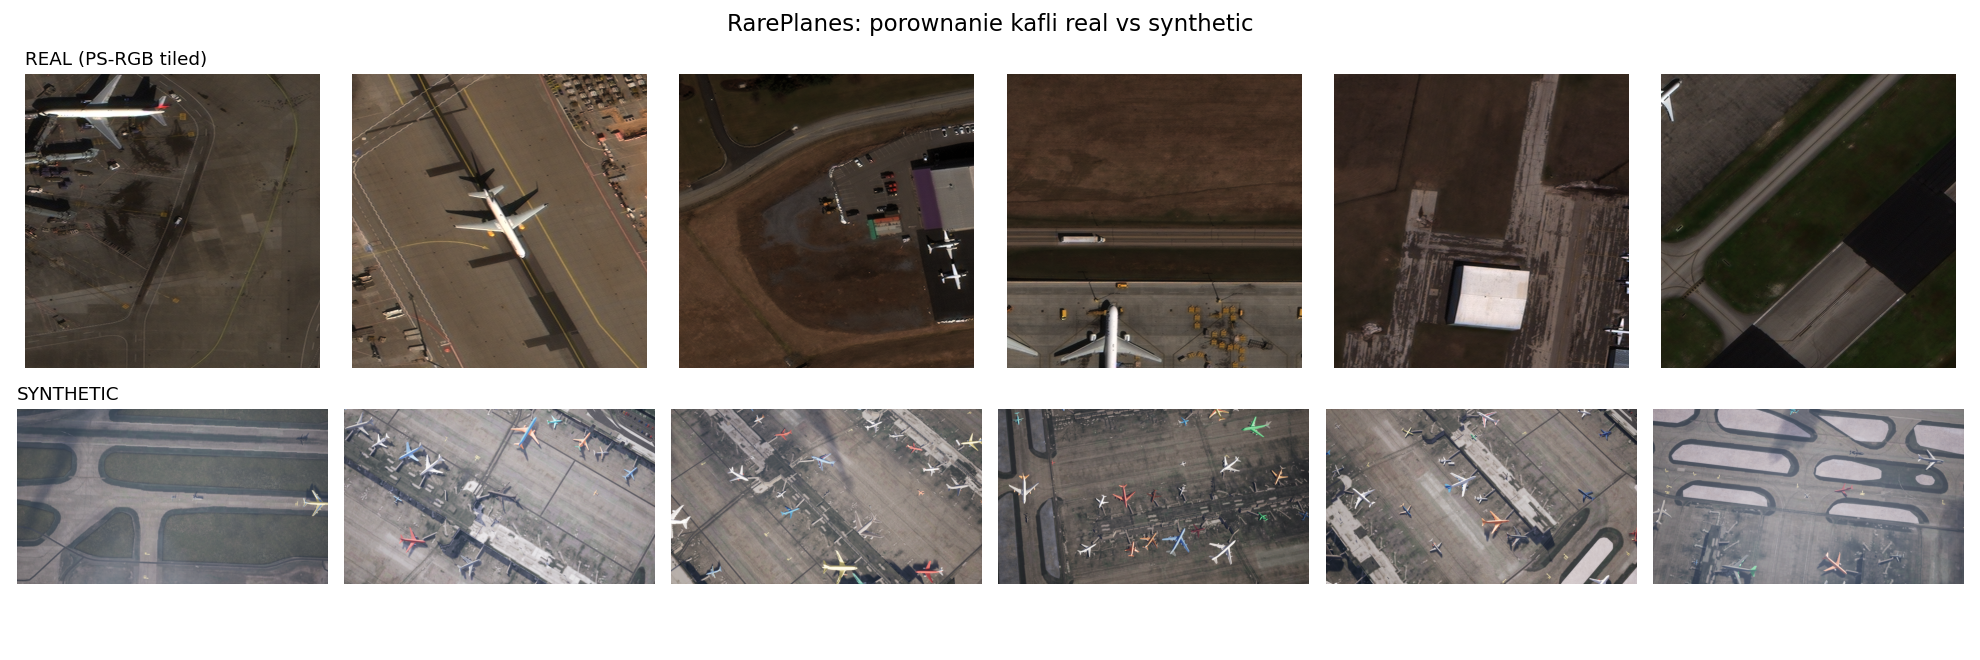
\includegraphics{../results/appearance/sample_tiles_real_vs_syn.png}

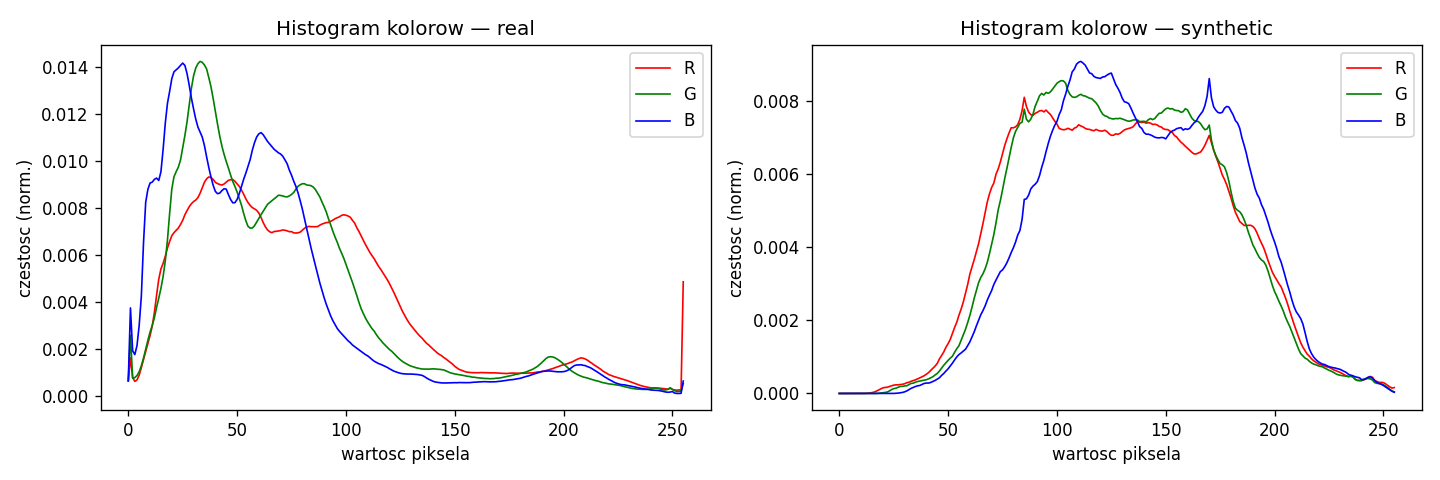
\includegraphics{../results/appearance/color_histograms.png}

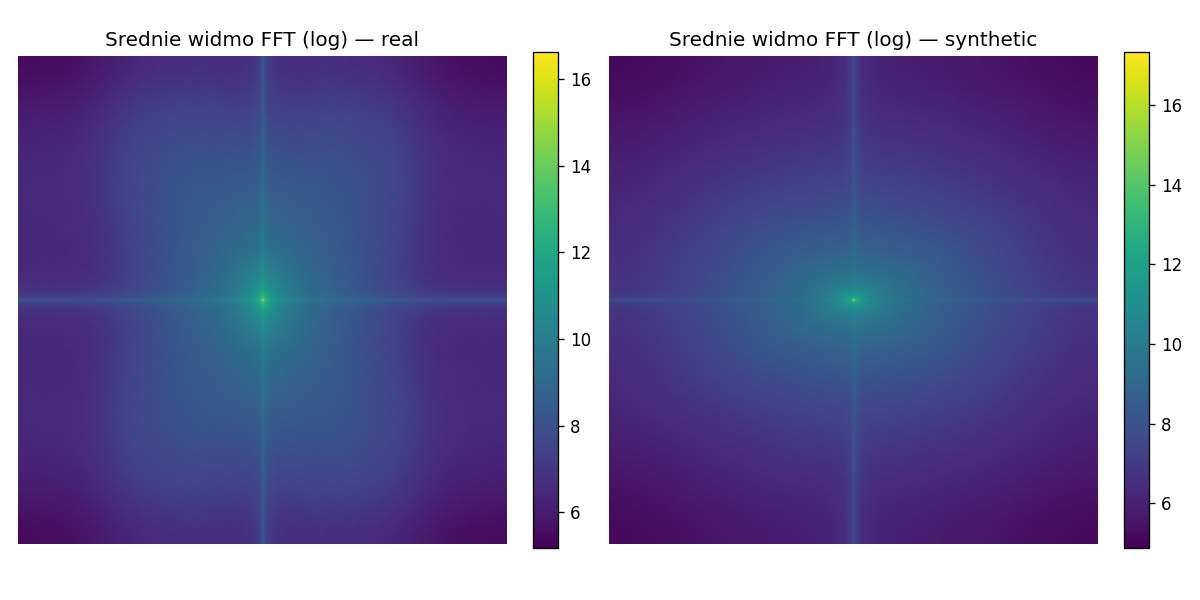
\includegraphics{../results/appearance/fft_spectra.png}

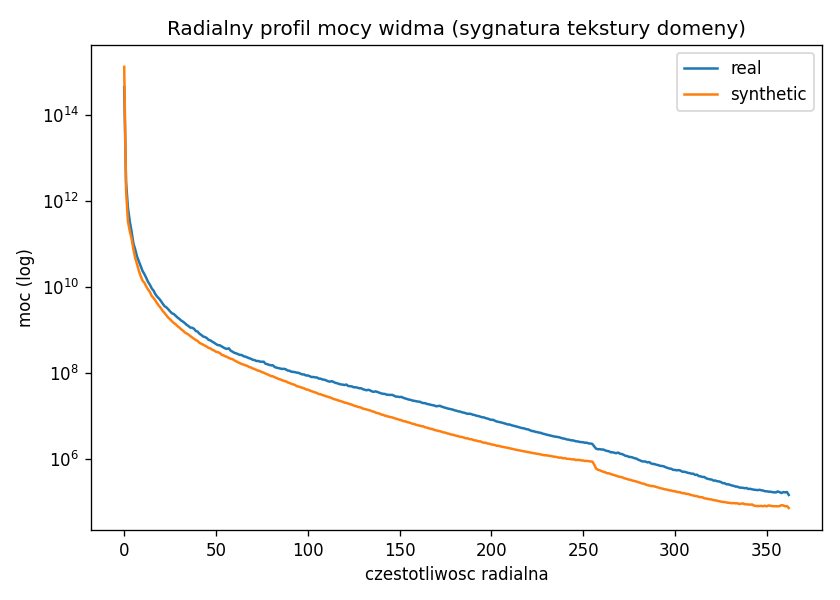
\includegraphics{../results/appearance/radial_power.png}

\hypertarget{metoda-i-protokuxf3ux142}{%
\subsection{Metoda i protokół}\label{metoda-i-protokuxf3ux142}}

Głównym modelem był \texttt{YOLOv10n}, startujący z wag pretrained COCO.
Dane RarePlanes w formacie COCO konwertowano do YOLO przez
\texttt{src/coco\_to\_yolo.py}. Trening wykonywał
\texttt{src/train\_yolo.py}, a ewaluację na realnym holdoucie
\texttt{src/eval\_per\_size.py} z użyciem metryk COCO i rozbiciem po
rozmiarach obiektów.

Główne metryki raportowe:

\begin{itemize}
\tightlist
\item
  \texttt{AP@.5},
\item
  \texttt{AP@{[}.5:.95{]}},
\item
  \texttt{AP\_small},
\item
  \texttt{AP\_medium},
\item
  \texttt{AP\_large},
\item
  \texttt{AR@100},
\item
  detekcje/obraz jako \texttt{n\_detections\ /\ 2710}.
\end{itemize}

Realny holdout testowy nie był używany do treningu ani do budowania
mixed-val. Wszystkie liczby w tabelach raportu pochodzą z ewaluacji COCO
na tym holdoucie (\texttt{results/per\_size/*.json}). Walidacja
Ultralytics/YOLO na zbiorach treningowych
(\texttt{results/baselines/*.json}) służyła wyłącznie jako kontrola
poprawności treningu i nie jest tu raportowana jako miara transferu ---
jej \texttt{mAP50} liczone na danych syntetycznych lub mieszanych nie
jest porównywalne z \texttt{AP@.5} na realnym teście. Oprócz AP
raportujemy liczbę detekcji na obraz (\texttt{n\_detections\ /\ 2710}),
bo samo AP nie pokazuje, że niektóre modele --- zwłaszcza synthetic 45k
i RT-DETR --- generują bardzo wielu kandydatów (do 300 na obraz), co
jest sygnałem słabej kalibracji na obcej domenie.

\begingroup
\rowcolors{2}{zebragray}{white}
\noindent\resizebox{\linewidth}{!}{%
\begin{tabular}{llrrr}
\toprule
Grupa wyników & Dane treningowe & Epoki & Batch & \texttt{imgsz} \\
\midrule

\bottomrule

Real baseline & real train/val & 100 & 64 & 512 \\
Synthetic 6460 & synthetic subset, 3 lotniska & 100 & 64 & 512 \\
Synthetic 45k & pełne synthetic 45k & 100 & 64 & 512 \\
A & synthetic 10k/45k + HSV & 60 / final 45k & różne & 512 \\
B & synthetic 10k po degradacji plikowej & 60 & 32 & 512 \\
C & synthetic 10k + real train/val & 30 & 32 & 512 \\
D & synthetic 10k, sweep skali & 45 & 16 & 320/768/1024 \\
Architektury & synthetic 10k & różne & różne & 512 \\
Final 45k & synthetic 45k B2 + real\_frac 0.25 + A1 & 60 & 64 & 320 \\
\end{tabular}%
}
\endgroup


Źródła metryk dla każdej grupy to odpowiadające pliki
\texttt{results/per\_size/*.json} (spis w sekcji „Artefakty w repo").

Rodziny eksperymentów A/B/C/D i porównanie architektur różnią się liczbą
obrazów, epok, wartościami \texttt{batch} i \texttt{imgsz} oraz
sprzętem. Dlatego ranking między rodzinami traktujemy jako praktyczne
porównanie skuteczności na realnym holdoucie, a mocniejsze wnioski
przyczynowe formułujemy wewnątrz pojedynczej rodziny, gdzie protokół
jest stały --- na przykład B2 wobec B1/B3 albo C 1/5/10/25\%.

\hypertarget{baseliney}{%
\subsection{Baseline\textquotesingle y}\label{baseliney}}

Baseline real-\textgreater real jest górnym punktem odniesienia:
pokazuje, co potrafi YOLOv10n, gdy dane treningowe i testowe są z tej
samej domeny. Baseline synthetic-\textgreater real mierzy właściwą lukę
domenową.

\begingroup
\rowcolors{2}{zebragray}{white}
\noindent\resizebox{\linewidth}{!}{%
\begin{tabular}{lrrrrrrr}
\toprule
Model & AP@.5 & AP@{[}.5:.95{]} & AP\_S & AP\_M & AP\_L & AR@100 &
Det/img \\
\midrule

\bottomrule

Real baseline & 0.9737 & 0.8073 & 0.7586 & 0.7825 & 0.8991 & 0.8465 &
9.5 \\
Synthetic 6460 & 0.4095 & 0.2388 & 0.2624 & 0.3284 & 0.0671 & 0.3686 &
33.8 \\
Synthetic 45k & 0.4525 & 0.2683 & 0.2859 & 0.3839 & 0.2008 & 0.5459 &
300.0 \\
\end{tabular}%
}
\endgroup


Przejście z 6460 syntetyków do pełnych 45k pomaga, ale umiarkowanie:
\texttt{AP@.5} rośnie z \texttt{0.4095} do \texttt{0.4525}, a
\texttt{AP@{[}.5:.95{]}} z \texttt{0.2388} do \texttt{0.2683}.
Największa poprawa pojawia się dla dużych obiektów (\texttt{AP\_large} z
\texttt{0.0671} do \texttt{0.2008}), co jest spójne z rozkładem danych
syntetycznych, gdzie duże obiekty są znacznie częstsze niż w realnym
train.

Równocześnie synthetic 45k zwraca maksymalne \texttt{300.0} detekcji na
obraz przy ewaluacji z niskim progiem confidence. To sugeruje model
mocno "rozgadany": poprawia recall, ale generuje bardzo dużo kandydatów.
Ta obserwacja jest niewidoczna, jeśli patrzymy wyłącznie na AP.

Skalę luki dobrze widać też na samej precyzji detektora. Ten sam model
synthetic 45k na walidacji syntetycznej osiąga precyzję \texttt{P=0.98}
i \texttt{mAP50=0.98}, natomiast na rzeczywistym holdoucie precyzja
spada do \texttt{P≈0.64} (\texttt{mAP50≈0.39} w mierze Ultralytics).
Rząd wielkości tego spadku --- z \textasciitilde98\% do
\textasciitilde64\% precyzji --- jest zgodny z oczekiwaniem, że naiwny
transfer z czystej syntetyki na zdjęcia rzeczywiste utrzymuje precyzję
rzędu zaledwie \textasciitilde60\%. Dopiero domieszka realnych próbek
(eksperyment C) i model finalny domykają tę różnicę.

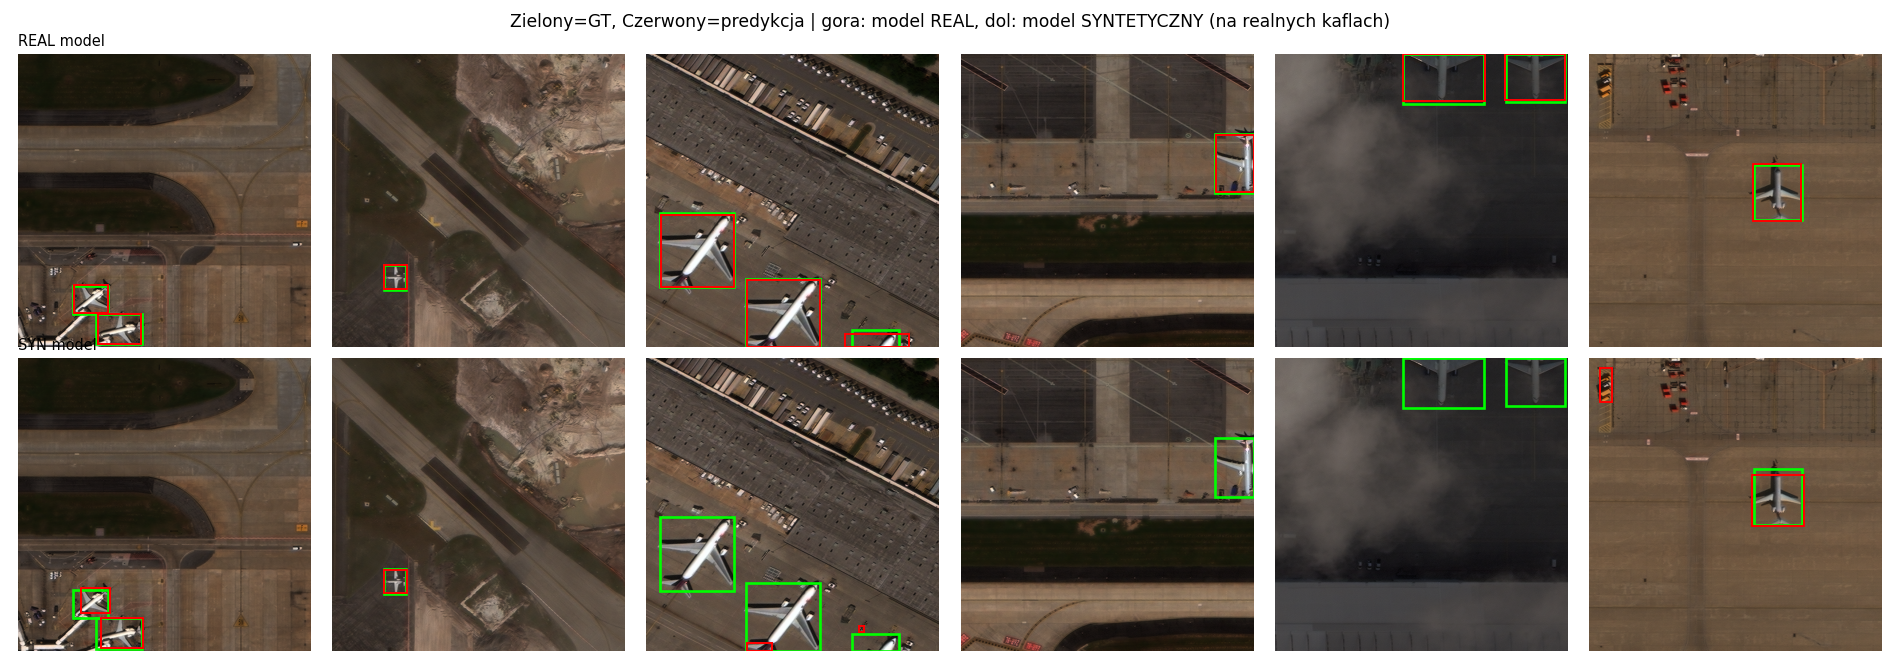
\includegraphics{../results/error_analysis_syn_vs_real.png}

\hypertarget{eksperyment-a-fotometria-hsv}{%
\subsection{Eksperyment A: fotometria
HSV}\label{eksperyment-a-fotometria-hsv}}

Eksperyment A sprawdzał, czy wzmocnienie augmentacji fotometrycznej
ograniczy różnice kolorystyczne między synthetic i real. Testowano
warianty HSV na 10k syntetyków oraz wariant A1 na pełniejszym treningu
45k.

\begingroup
\rowcolors{2}{zebragray}{white}
\noindent\resizebox{\linewidth}{!}{%
\begin{tabular}{llrrrrrr}
\toprule
Wariant & Opis & AP@.5 & AP@{[}.5:.95{]} & AP\_S & AP\_M & AP\_L &
AR@100 \\
\midrule

\bottomrule

Synthetic 45k baseline & bez A1 & 0.4525 & 0.2683 & 0.2859 & 0.3839 &
0.2008 & 0.5459 \\
A1 weak 10k & łagodne HSV & 0.4591 & 0.2643 & 0.3056 & 0.3571 & 0.0908 &
0.3970 \\
A2 medium 10k & mocniejsze HSV & 0.4308 & 0.2469 & 0.2646 & 0.3447 &
0.0986 & 0.3931 \\
A3 strong 10k & silne HSV & 0.4463 & 0.2520 & 0.2679 & 0.3443 & 0.1052 &
0.3941 \\
A1 weak 45k & finalny wariant A & 0.4549 & 0.2684 & 0.3370 & 0.3545 &
0.0902 & 0.4043 \\
\end{tabular}%
}
\endgroup


A1 jest najlepszym ustawieniem HSV w tej rodzinie, ale globalny zysk
jest marginalny. Na 45k \texttt{AP@.5} rośnie tylko z \texttt{0.4525} do
\texttt{0.4549}, a \texttt{AP@{[}.5:.95{]}} praktycznie się nie zmienia.
Ważniejsza jest redystrybucja jakości: \texttt{AP\_small} rośnie z
\texttt{0.2859} do \texttt{0.3370}, ale \texttt{AP\_large} spada z
\texttt{0.2008} do \texttt{0.0902}.

Wniosek: HA jest potwierdzona słabo. Fotometria pomaga małym obiektom,
ale nie domyka globalnej luki domenowej i może pogorszyć detekcję dużych
obiektów.

\hypertarget{eksperyment-b-degradacja-czux119stotliwoux15bciowa}{%
\subsection{Eksperyment B: degradacja
częstotliwościowa}\label{eksperyment-b-degradacja-czux119stotliwoux15bciowa}}

Eksperyment B wynikał z analizy FFT: realne zdjęcia zawierały więcej
wysokich częstotliwości niż gładkie syntetyki. Testowano degradacje
materializowane do plików, a nie wersję on-the-fly, ponieważ
wcześniejsze uruchomienie on-the-fly okazało się niewiarygodne i nie
jest źródłem wyników raportowych.

\begingroup
\rowcolors{2}{zebragray}{white}
\noindent\resizebox{\linewidth}{!}{%
\begin{tabular}{llrrrrrrr}
\toprule
Wariant & Degradacja & AP@.5 & AP@{[}.5:.95{]} & AP\_S & AP\_M & AP\_L &
AR@100 & Det/img \\
\midrule

\bottomrule

B1 & blur + noise & 0.4515 & 0.2585 & 0.2611 & 0.3579 & 0.1006 & 0.3999
& 30.0 \\
B2 & noise only, \texttt{sigma=8} & 0.4897 & 0.2797 & 0.2829 & 0.3821 &
0.1190 & 0.4353 & 44.2 \\
B3 & blur + noise + JPEG & 0.4509 & 0.2610 & 0.2943 & 0.3558 & 0.1009 &
0.4031 & 41.7 \\
\end{tabular}%
}
\endgroup


Najlepszy jest B2, czyli sam szum. Blur nie pomaga, a w praktyce kasuje
wysokie częstotliwości, których właśnie brakuje syntetykom względem
realnych zdjęć. B3 poprawia \texttt{AP\_small} względem B1, ale
globalnie nie przebija B2.

Wniosek: HB jest potwierdzona częściowo. Pomaga dodanie szumu, nie
pomaga rozmycie. Dlatego finalny model używa tylko B2:
\texttt{noise\_sigma=8.0}, bez blur i bez JPEG.

\hypertarget{eksperyment-c-mixed-training}{%
\subsection{Eksperyment C: mixed
training}\label{eksperyment-c-mixed-training}}

Eksperyment C jest najważniejszy jakościowo. Sprawdzał, jak dodanie
części realnego train/val do syntetyki wpływa na transfer na realny
holdout testowy.

Warto doprecyzować, co oznacza \texttt{real\_frac}: jest to procent
dostępnego realnego splitu train/val dołączonego do syntetyki, a nie
procent realnych obrazów w finalnym zbiorze mieszanym. Realny test nigdy
nie był dodawany do treningu ani walidacji mixed.

\begingroup
\rowcolors{2}{zebragray}{white}
\begin{tabularx}{\linewidth}{LRRRRRR}
\toprule
Wariant & Train synthetic & Train real & Real share train & Val
synthetic & Val real & Real share val \\
\midrule

\bottomrule

C 1\% & 10 000 & 49 / 4 943 & 0.49\% & 1 764 & 9 / 872 & 0.51\% \\
C 5\% & 10 000 & 247 / 4 943 & 2.41\% & 1 764 & 44 / 872 & 2.43\% \\
C 10\% & 10 000 & 494 / 4 943 & 4.71\% & 1 764 & 87 / 872 & 4.70\% \\
C 25\% & 10 000 & 1 236 / 4 943 & 11.00\% & 1 764 & 218 / 872 &
11.00\% \\
\end{tabularx}
\endgroup


Wszystkie główne warianty C trenowano jako \texttt{YOLOv10n},
\texttt{epochs=30}, \texttt{batch=32}, \texttt{imgsz=512},
\texttt{workers=4}, \texttt{seed=42}, z domyślną augmentacją
Ultralytics. C nie używał B2 ani A1; badał przede wszystkim skład
danych.

\begingroup
\rowcolors{2}{zebragray}{white}
\noindent\resizebox{\linewidth}{!}{%
\begin{tabular}{lrrrrrrr}
\toprule
Wariant & AP@.5 & AP@{[}.5:.95{]} & AP\_S & AP\_M & AP\_L & AR@100 &
Det/img \\
\midrule

\bottomrule

C 1\% & 0.6666 & 0.3957 & 0.3614 & 0.4535 & 0.3462 & 0.5954 & 66.5 \\
C 5\% & 0.8516 & 0.5660 & 0.5197 & 0.5761 & 0.6108 & 0.7144 & 39.4 \\
C 10\% & 0.8960 & 0.6188 & 0.5404 & 0.6184 & 0.7060 & 0.7349 & 35.6 \\
C 25\% & 0.9466 & 0.7120 & 0.6365 & 0.6974 & 0.8166 & 0.7822 & 20.8 \\
\end{tabular}%
}
\endgroup


Krzywa jest monotoniczna: każda większa dawka realnych danych poprawia
wynik na realnym holdoucie. Równocześnie spada liczba detekcji na obraz,
zwłaszcza od C 1\% do C 25\%, co sugeruje lepszą kalibrację i mniej
fałszywych kandydatów.

C 25\% zbliża się do real baseline w \texttt{AP@.5}: \texttt{0.9466}
wobec \texttt{0.9737}. Nadal pozostaje luka w \texttt{AP@{[}.5:.95{]}} i
\texttt{AP\_small}, ale w praktyce to najlepszy wynik synthetic+real w
projekcie. HC jest mocno potwierdzona: realne próbki są najsilniejszą
kotwicą domenową.

\hypertarget{eksperyment-d-skala-wejux15bcia}{%
\subsection{Eksperyment D: skala
wejścia}\label{eksperyment-d-skala-wejux15bcia}}

Eksperyment D sprawdzał hipotezę skali. Pierwotna intuicja była taka, że
większa rozdzielczość wejścia pomoże małym obiektom. Wynik był odwrotny:
najlepsze okazało się \texttt{imgsz=320}.

\begingroup
\rowcolors{2}{zebragray}{white}
\noindent\resizebox{\linewidth}{!}{%
\begin{tabular}{rrrrrrrrl}
\toprule
\texttt{imgsz} & AP@.5 & AP@{[}.5:.95{]} & AP\_S & AP\_M & AP\_L &
AR@100 & Det/img & Status \\
\midrule

\bottomrule

320 & 0.5224 & 0.2828 & 0.3078 & 0.3675 & 0.1511 & 0.4358 & 54.2 &
główny wariant D \\
512 & 0.4591 & 0.2643 & 0.3056 & 0.3571 & 0.0908 & 0.3970 & 27.4 & punkt
referencyjny, nie osobny \texttt{expD\_512\_*} \\
768 & 0.4476 & 0.2519 & 0.2299 & 0.3390 & 0.1162 & 0.3741 & 14.8 &
główny wariant D \\
1024 & 0.3297 & 0.1895 & 0.2222 & 0.2500 & 0.0474 & 0.2839 & 7.4 &
główny wariant D \\
\end{tabular}%
}
\endgroup


Wniosek jest mechanicznie spójny z analizą adnotacji. Syntetyczne
samoloty są większe niż realne, więc downscaling podczas treningu działa
jak implicytne dopasowanie rozkładu skali. Zwiększanie rozdzielczości
utrwala różnicę: model jeszcze silniej widzi syntetyczne samoloty jako
duże i wyraźne, a potem gorzej transferuje na mniejsze realne obiekty.

HD została więc potwierdzona odwrotnie: skala pomaga, ale przez
zmniejszenie wejścia, nie przez powiększenie. Trzeba jednak zachować
ostrożność: punkt \texttt{512} jest referencją z innego przebiegu 10k, a
nie pełnoprawnym wariantem tego samego sweepa D.

\hypertarget{poruxf3wnanie-architektur}{%
\subsection{Porównanie architektur}\label{poruxf3wnanie-architektur}}

Porównanie architektur sprawdzało, czy większy albo nowszy model lepiej
zniesie domain shift. Wyniki nie potwierdziły prostej zależności
"większy model = lepszy transfer".

\begingroup
\rowcolors{2}{zebragray}{white}
\noindent\resizebox{\linewidth}{!}{%
\begin{tabular}{llrrrrrrrr}
\toprule
Model & Typ & Parametry & AP@.5 & AP@{[}.5:.95{]} & AP\_S & AP\_M &
AP\_L & AR@100 & Det/img \\
\midrule

\bottomrule

YOLO11l & CNN & ok. 25M & 0.4670 & 0.2708 & 0.3061 & 0.3483 & 0.1081 &
0.3922 & 22.6 \\
YOLOv10n & CNN & ok. 2.3M & 0.4591 & 0.2643 & 0.3056 & 0.3571 & 0.0908 &
0.3970 & 27.4 \\
RT-DETR-x & Transformer & ok. 67M & 0.3796 & 0.2051 & 0.2058 & 0.2849 &
0.0942 & 0.3731 & 300.0 \\
RT-DETR-l & Transformer & ok. 32M & 0.2973 & 0.1575 & 0.1462 & 0.2296 &
0.0807 & 0.3076 & 300.0 \\
\end{tabular}%
}
\endgroup


CNN-y transferują lepiej niż RT-DETR w tym setupie. YOLO11l lekko
przebija YOLOv10n, ale różnica jest dużo mniejsza niż zyski z C lub D.
RT-DETR-x jest lepszy od RT-DETR-l, więc nie jest prawdą, że większy
transformer był gorszy od mniejszego. Problemem jest raczej mechanizm
detekcji end-to-end i kalibracja na obcej domenie: oba RT-DETR zwróciły
\texttt{300.0} detekcji na obraz, czyli wykorzystały wszystkie sloty
zapytań.

Wniosek HArch: architektura ma znaczenie, ale w tym projekcie zmiana
architektury była słabszą dźwignią niż skład danych. Najważniejsza nie
była pojemność modelu, tylko odporność mechanizmu detekcji i selekcji
kandydatów na domain shift.

\hypertarget{grad-cam--eigencam}{%
\subsection{Grad-CAM / EigenCAM}\label{grad-cam--eigencam}}

Interpretowalność wykonano przez EigenCAM na warstwie 8 backbone
YOLOv10n, czyli bloku C2f o rozdzielczości przestrzennej \texttt{16x16}.
Klasyczny Grad-CAM jest mniej naturalny dla YOLOv10, ponieważ model
detekcyjny end-to-end nie daje pojedynczego skalaru klasy w taki sam
sposób jak klasyfikator. Skrypt \texttt{src/gradcam\_compare.py}
porównuje uwagę sześciu modeli na tych samych realnych kaflach z małymi
obiektami.

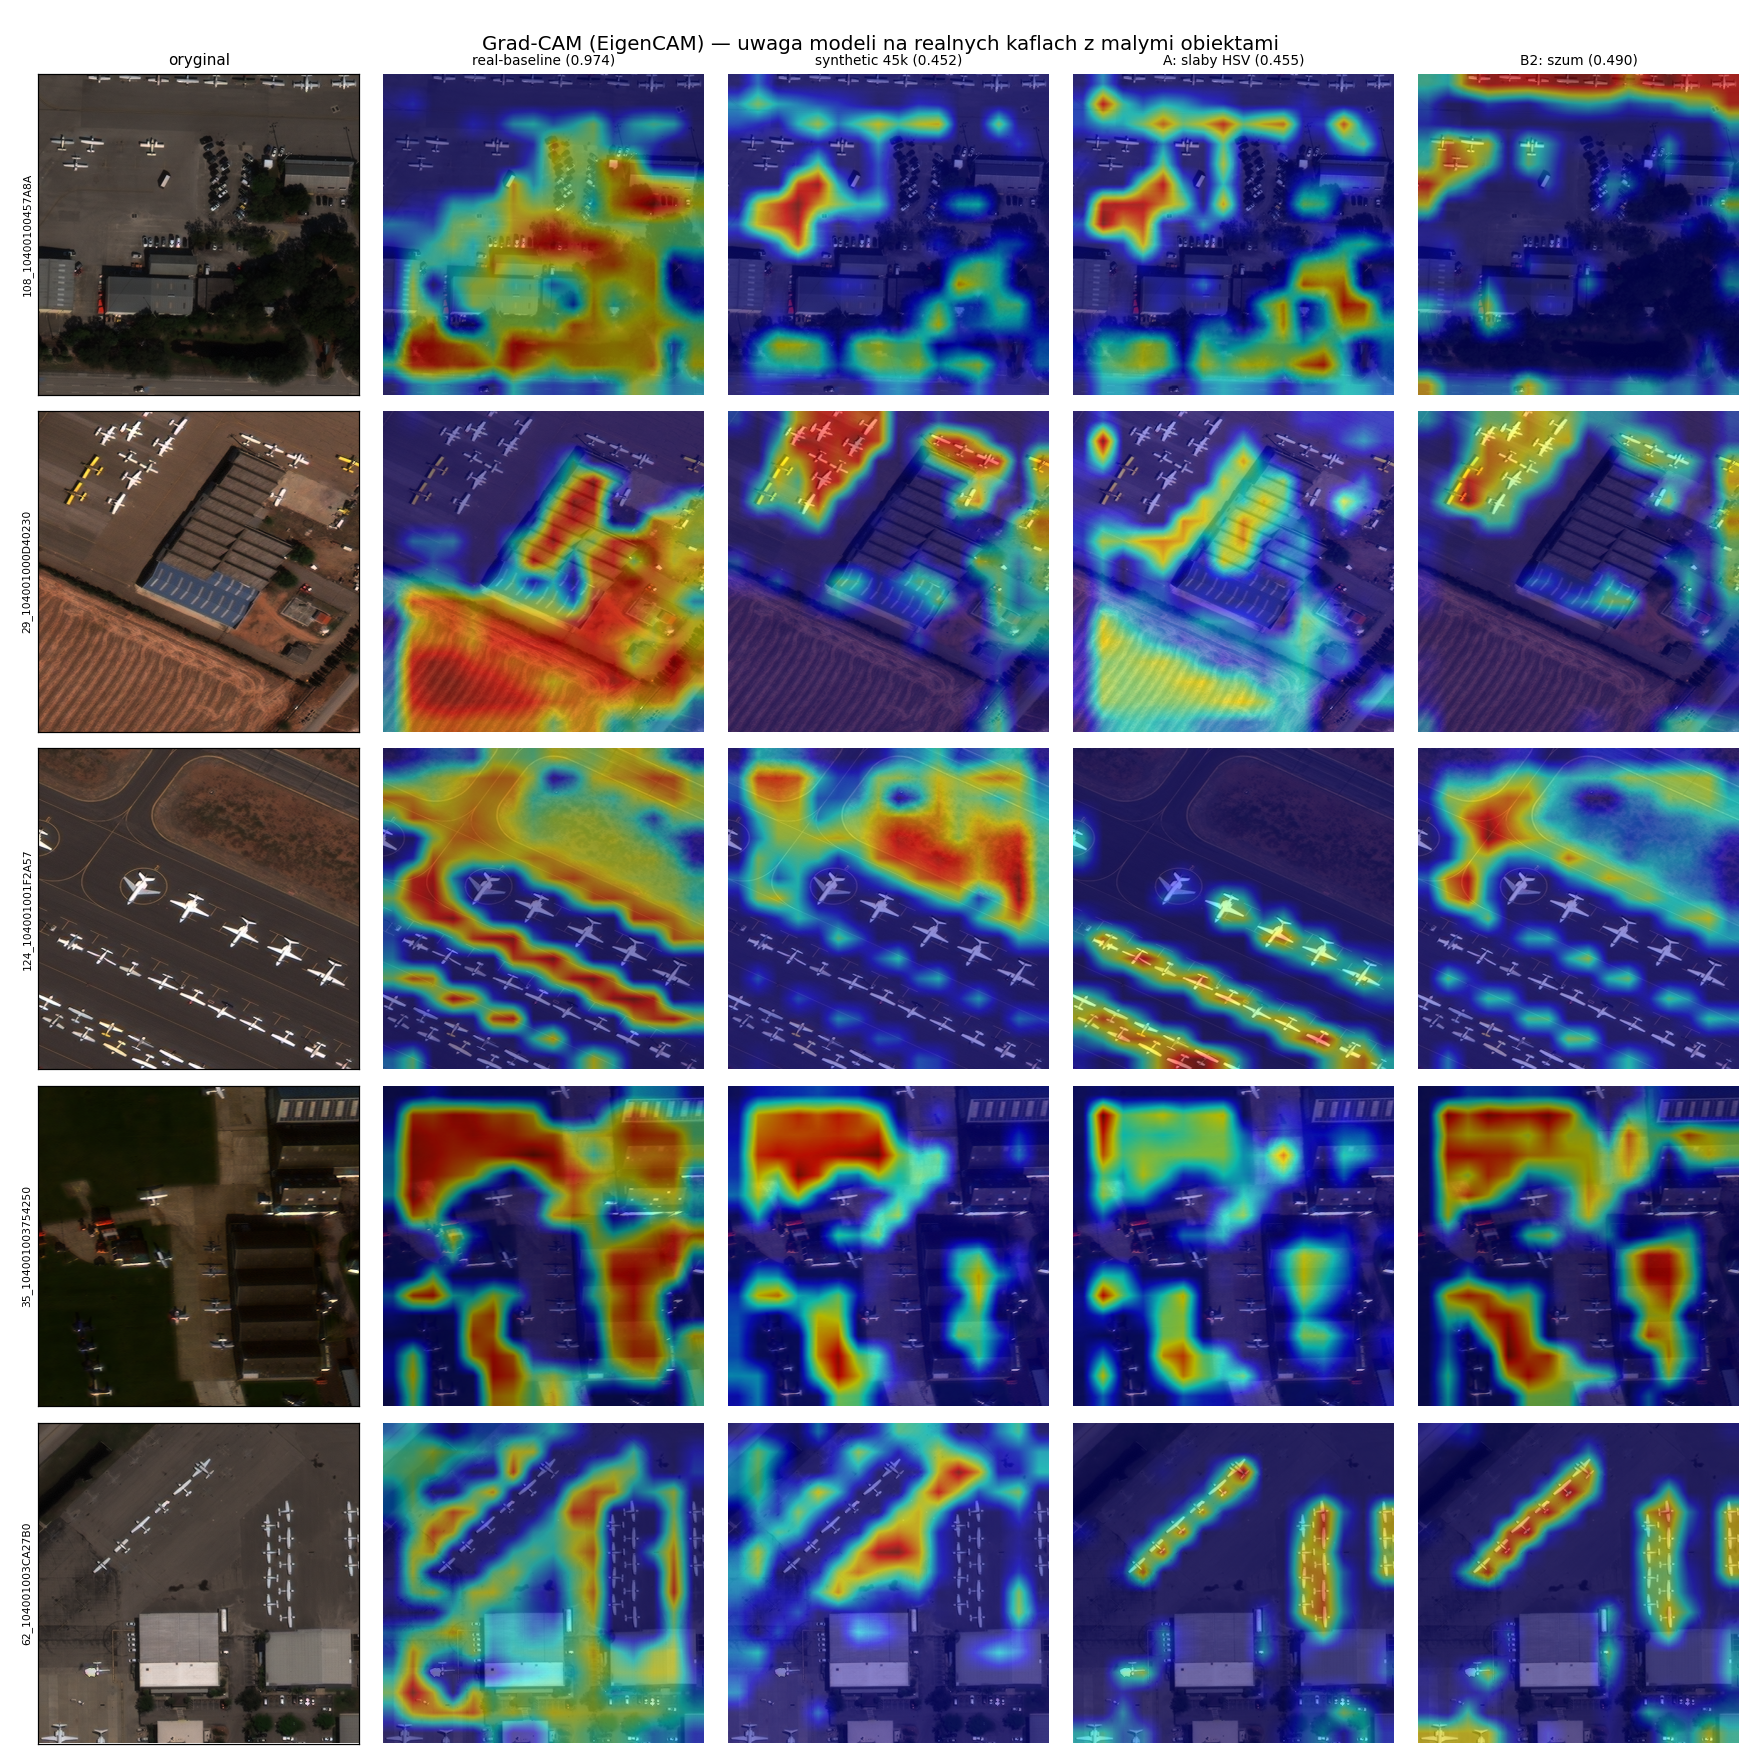
\includegraphics{../results/gradcam/gradcam_comparison.png}

Wzorce jakościowe:

\begin{itemize}
\tightlist
\item
  model real baseline ma uwagę bardziej rozlaną po scenie, w tym po
  kontekście lotniska;
\item
  modele synthetic, A i B2 częściej skupiają się na strukturach
  liniowych i rzędach samolotów;
\item
  B2 ma bardziej precyzyjną aktywację na rzędach małych samolotów niż
  czysty synthetic baseline;
\item
  D \texttt{imgsz=320} pokazuje bardziej skupioną uwagę na obiektach niż
  baseline synthetic, co pasuje do mechanizmu dopasowania skali;
\item
  C 25\% przesuwa uwagę w stronę real baseline, czyli realne próbki
  zmieniają reprezentację, a nie tylko podbijają metrykę.
\end{itemize}

Najważniejszy wniosek jakościowy jest pozytywny: modele syntetyczne nie
ignorują małych realnych samolotów i nie skupiają się wyłącznie na tle
lub artefaktach renderu. Luka domenowa wynika raczej z różnic rozkładu
rozmiarów, gęstości, fotometrii i tekstury niż z całkowitego nauczenia
się błędnych cech.

Ograniczenie: EigenCAM nie dowodzi mechanizmu przyczynowego i nie
powinien być używany jako metryka. Liczby przy figurze są orientacyjne,
a tabele raportowe korzystają z JSON-ów per-size.

\hypertarget{model-finalny-45k}{%
\subsection{Model finalny 45k}\label{model-finalny-45k}}

Model finalny miał sprawdzić, co stanie się po połączeniu najlepszych
decyzji projektowych w jednym treningu na pełnej syntetyce 45k.

Receptura:

\begin{Shaded}
\begin{Highlighting}[]
\NormalTok{B2 + C + D + A1}
\end{Highlighting}
\end{Shaded}

Szczegóły:

\begingroup
\rowcolors{2}{zebragray}{white}
\noindent\resizebox{\linewidth}{!}{%
\begin{tabular}{ll}
\toprule
Element & Wartość \\
\midrule

\bottomrule

Run & \texttt{final\_yolov10n\_syn45k\_noise\_}
\texttt{real25pct\_img320\_hsvA1\_ml} \\
Architektura & \texttt{yolov10n.pt} \\
Synthetic & pełne 45k, po B2 \\
B2 & \texttt{noise\_sigma=8.0}, \texttt{blur\_radius=0.0},
\texttt{jpeg\_quality\_min=None} \\
C & \texttt{real\_frac=0.25} dostępnego real train/val \\
D & \texttt{imgsz=320} \\
A1 & \texttt{hsv\_h=0.015}, \texttt{hsv\_s=0.4}, \texttt{hsv\_v=0.3} \\
Epoki & 60 \\
Batch & 64 \\
Workers & 4 \\
Seed & 42 \\
Uruchomienie & \texttt{run\_train\_final\_cluster.sh} \\
Log & \texttt{train-final-75379.out} \\
\end{tabular}%
}
\endgroup


Rzeczywisty skład danych:

\begingroup
\rowcolors{2}{zebragray}{white}
\begin{tabularx}{\linewidth}{LRRRR}
\toprule
Split & Synthetic & Real & Razem & Udział real \\
\midrule

\bottomrule

train & 38 250 & 1 236 / 4 943 & 39 486 & 3.13\% \\
val & 6 750 & 218 / 872 & 6 968 & 3.13\% \\
\end{tabularx}
\endgroup


Ta tabela wyjaśnia główny paradoks finalnego modelu. Final używa pełnych
45k syntetyków, ale ta sama liczba realnych obrazów, która w C 25\%
stanowiła około 11\% treningu, tutaj stanowi tylko około 3.13\%. Realny
sygnał zostaje rozcieńczony przez syntetykę.

Wyniki:

\begingroup
\rowcolors{2}{zebragray}{white}
\noindent\resizebox{\linewidth}{!}{%
\begin{tabular}{lrrrrrrr}
\toprule
Model & AP@.5 & AP@{[}.5:.95{]} & AP\_S & AP\_M & AP\_L & AR@100 &
Det/img \\
\midrule

\bottomrule

Synthetic 45k baseline & 0.4525 & 0.2683 & 0.2859 & 0.3839 & 0.2008 &
0.5459 & 300.0 \\
C 25\% real 10k & 0.9466 & 0.7120 & 0.6365 & 0.6974 & 0.8166 & 0.7822 &
20.8 \\
Final 45k B2+C+D+A1 & 0.9031 & 0.6332 & 0.5616 & 0.6179 & 0.7523 &
0.7480 & 28.8 \\
Real baseline & 0.9737 & 0.8073 & 0.7586 & 0.7825 & 0.8991 & 0.8465 &
9.5 \\
\end{tabular}%
}
\endgroup


Finalny model bardzo poprawia synthetic 45k: \texttt{AP@.5} rośnie z
\texttt{0.4525} do \texttt{0.9031}, \texttt{AP@{[}.5:.95{]}} z
\texttt{0.2683} do \texttt{0.6332}, a liczba detekcji spada z
\texttt{300.0} do \texttt{28.8} na obraz. To duży sukces praktyczny.

Nie jest to jednak najlepszy model synthetic+real w projekcie. C 25\%
10k jest lepszy w każdej głównej metryce: \texttt{AP@.5=0.9466} kontra
\texttt{0.9031}, \texttt{AP@{[}.5:.95{]}=0.7120} kontra \texttt{0.6332},
\texttt{AP\_small=0.6365} kontra \texttt{0.5616}. Model finalny pokazuje
więc ograniczenie addytywności: B2, C, D i A1 były sensowne osobno, ale
ich połączenie z większą syntetyką zmieniło proporcję danych i nie dało
najlepszego wyniku.

Benchmark finalnego modelu z
\texttt{results/final\_combined\_model\_summary.md}:

\begingroup
\rowcolors{2}{zebragray}{white}
\begin{tabularx}{\linewidth}{LR}
\toprule
Cecha & Wartość \\
\midrule

\bottomrule

FPS & 100.79 \\
Peak CUDA memory & 1340.7 MB \\
Obrazy benchmarku & 256 \\
\end{tabularx}
\endgroup


Model finalny jest szybki i lekki, więc pozostaje praktycznie użyteczny,
nawet jeśli nie jest zwycięzcą jakościowym.

\hypertarget{synteza-hipotez}{%
\subsection{Synteza hipotez}\label{synteza-hipotez}}

\begingroup
\rowcolors{2}{zebragray}{white}
\noindent\resizebox{\linewidth}{!}{%
\begin{tabular}{llll}
\toprule
Hipoteza & Status & Najważniejszy dowód & Wniosek \\
\midrule

\bottomrule

HA fotometria & słabo/częściowo potwierdzona & A1 45k:
\texttt{AP@.5=0.4549} vs synthetic 45k \texttt{0.4525};
\texttt{AP\_small} rośnie do \texttt{0.3370} & HSV pomaga małym
obiektom, ale globalnie prawie nie domyka luki. \\
HB częstotliwości & częściowo potwierdzona & B2: \texttt{AP@.5=0.4897},
B1/B3 około \texttt{0.451} & Pomaga szum, nie pomaga blur. \\
HC mixed training & mocno potwierdzona & C 25\%: \texttt{AP@.5=0.9466},
\texttt{AP@{[}.5:.95{]}=0.7120} & Realne próbki są najsilniejszą kotwicą
domenową. \\
HD skala & potwierdzona odwrotnie & D 320: \texttt{AP@.5=0.5224}; D
1024: \texttt{0.3297} & Mniejsze \texttt{imgsz} działa jak dopasowanie
skali synthetic do real. \\
HArch architektura & potwierdzona częściowo & YOLO11l \texttt{0.4670},
RT-DETR-x \texttt{0.3796}, RT-DETR-l \texttt{0.2973} & CNN-y były
odporniejsze niż RT-DETR, ale skład danych był ważniejszy niż
architektura. \\
\end{tabular}%
}
\endgroup


Praktyczny ranking jakościowy na realnym holdoucie:

\begin{Shaded}
\begin{Highlighting}[]
\NormalTok{C 25\% real 10k \textgreater{} final 45k B2+C+D+A1 \textgreater{} C 10\% \textgreater{} C 5\% \textgreater{} C 1\%}
\NormalTok{\textgreater{} D 320 \textgreater{} B2 noise \textgreater{} A1 HSV \textasciitilde{}= synthetic 45k \textgreater{}\textgreater{} RT{-}DETR{-}l}
\end{Highlighting}
\end{Shaded}

Ranking czysto syntetycznych interwencji:

\begin{Shaded}
\begin{Highlighting}[]
\NormalTok{D imgsz320 \textgreater{} B2 noise \textgreater{} A1 HSV \textasciitilde{}= synthetic 45k baseline}
\end{Highlighting}
\end{Shaded}

Najważniejszy wniosek naukowy: zwiększenie liczby syntetyków pomaga, ale
nie zastępuje realnych próbek. Najważniejszy wniosek inżynierski: jeśli
budżet adnotacyjny jest mały, warto przeznaczyć go na choćby kilka
procent realnych przykładów, zanim zacznie się kosztownie generować i
trenować na dużo większej liczbie syntetyków.

\hypertarget{ograniczenia}{%
\subsection{Ograniczenia}\label{ograniczenia}}

\begin{enumerate}
\def\labelenumi{\arabic{enumi}.}
\tightlist
\item
  Większość eksperymentów wykonano dla jednego seeda (\texttt{42}). Małe
  różnice, zwłaszcza w A, mogą być porównywalne z wariancją treningu.
\item
  Rodziny eksperymentów różnią się protokołem: C ma 30 epok i mixed
  data, D ma sweep skali, final ma 60 epok i 45k synthetic. Globalne
  porównania są praktyczne, nie w pełni przyczynowe.
\item
  Część wyników liczono na różnych GPU i środowiskach. FPS-y między
  rodzinami nie powinny być porównywane bez wspólnego benchmarku.
\item
  Nazwę \texttt{real25pct} należy czytać jako 25\% dostępnego real
  train/val, a nie jako udział realnych obrazów w finalnym zbiorze
  mieszanym.
\item
  Mixed-val nie jest główną metryką. Wyniki mixed-val mogą być wysokie i
  nie dowodzą transferu na realny holdout.
\item
  Grad-CAM/EigenCAM jest jakościowy. Nie należy z niego wyprowadzać
  liczbowych rankingów.
\item
  Punkt \texttt{imgsz=512} w sekcji D jest referencją, a nie osobnym
  plikiem \texttt{expD\_512\_*}.
\item
  Dane i checkpointy są ciężkie i nie są redystrybuowane w repo. Pełna
  reprodukcja wymaga pobrania RarePlanes oraz odtworzenia treningów.
\item
  Final 45k nie dowodzi, że wszystkie dobre interwencje się sumują.
  Pokazuje raczej, że proporcja realnego sygnału może przeważyć nad
  skalą syntetyki.
\end{enumerate}

\hypertarget{reprodukcja}{%
\subsection{Reprodukcja}\label{reprodukcja}}

Poniższe komendy są skrótem najważniejszych ścieżek. Szczegóły
konkretnych uruchomień są w notatkach i logach.

Przygotowanie danych i konwersja:

\begin{Shaded}
\begin{Highlighting}[]
\ExtensionTok{python}\NormalTok{ src/coco\_to\_yolo.py }\AttributeTok{{-}{-}domain}\NormalTok{ synthetic }\AttributeTok{{-}{-}classes}\NormalTok{ aircraft }\AttributeTok{{-}{-}val{-}frac}\NormalTok{ 0.15}
\ExtensionTok{python}\NormalTok{ src/coco\_to\_yolo.py }\AttributeTok{{-}{-}domain}\NormalTok{ real }\AttributeTok{{-}{-}classes}\NormalTok{ aircraft}
\ExtensionTok{python}\NormalTok{ src/make\_subset.py }\AttributeTok{{-}{-}n{-}train}\NormalTok{ 10000 }\AttributeTok{{-}{-}name}\NormalTok{ synthetic\_10k}
\end{Highlighting}
\end{Shaded}

Ewaluacja per-size na realnym holdoucie:

\begin{Shaded}
\begin{Highlighting}[]
\ExtensionTok{python}\NormalTok{ src/eval\_per\_size.py }\DataTypeTok{\textbackslash{}}
  \AttributeTok{{-}{-}weights}\NormalTok{ runs/}\OperatorTok{\textless{}}\NormalTok{run}\OperatorTok{\textgreater{}}\NormalTok{/weights/best.pt }\DataTypeTok{\textbackslash{}}
  \AttributeTok{{-}{-}img{-}dir}\NormalTok{ data/real/PS{-}RGB\_tiled/PS{-}RGB\_tiled }\DataTypeTok{\textbackslash{}}
  \AttributeTok{{-}{-}coco{-}gt}\NormalTok{ data/real/annotations/instances\_test\_aircraft.json }\DataTypeTok{\textbackslash{}}
  \AttributeTok{{-}{-}name} \OperatorTok{\textless{}}\NormalTok{run}\OperatorTok{\textgreater{}}
\end{Highlighting}
\end{Shaded}

Eksperyment C na klastrze:

\begin{Shaded}
\begin{Highlighting}[]
\ExtensionTok{sbatch}\NormalTok{ src/run\_expC.sh}
\end{Highlighting}
\end{Shaded}

Najważniejsze parametry C:

\begin{Shaded}
\begin{Highlighting}[]
\ExtensionTok{python}\NormalTok{ src/expC.py }\DataTypeTok{\textbackslash{}}
  \AttributeTok{{-}{-}data{-}dir}\NormalTok{ /work/}\VariableTok{$USER}\NormalTok{/rareplanes{-}data/data }\DataTypeTok{\textbackslash{}}
  \AttributeTok{{-}{-}batch}\NormalTok{ 32 }\DataTypeTok{\textbackslash{}}
  \AttributeTok{{-}{-}workers}\NormalTok{ 4 }\DataTypeTok{\textbackslash{}}
  \AttributeTok{{-}{-}device}\NormalTok{ 0 }\DataTypeTok{\textbackslash{}}
  \AttributeTok{{-}{-}epochs}\NormalTok{ 30}
\end{Highlighting}
\end{Shaded}

Model finalny na klastrze:

\begin{Shaded}
\begin{Highlighting}[]
\ExtensionTok{sbatch}\NormalTok{ run\_train\_final\_cluster.sh}
\end{Highlighting}
\end{Shaded}

Skrypt \texttt{run\_train\_final\_cluster.sh} uruchamia:

\begin{Shaded}
\begin{Highlighting}[]
\ExtensionTok{python}\NormalTok{ src/train\_final\_model.py }\DataTypeTok{\textbackslash{}}
  \AttributeTok{{-}{-}data{-}dir}\NormalTok{ /work/}\VariableTok{$\{USER\}}\NormalTok{/rareplanes{-}data/data }\DataTypeTok{\textbackslash{}}
  \AttributeTok{{-}{-}epochs}\NormalTok{ 60 }\DataTypeTok{\textbackslash{}}
  \AttributeTok{{-}{-}batch}\NormalTok{ 64 }\DataTypeTok{\textbackslash{}}
  \AttributeTok{{-}{-}workers}\NormalTok{ 4 }\DataTypeTok{\textbackslash{}}
  \AttributeTok{{-}{-}device}\NormalTok{ 0 }\DataTypeTok{\textbackslash{}}
  \AttributeTok{{-}{-}full{-}download{-}workers}\NormalTok{ 32}
\end{Highlighting}
\end{Shaded}

Pipeline finalny wykonuje przygotowanie danych, materializację B2,
zbudowanie mixed datasetu, trening YOLOv10n, ewaluację na realnym
holdoucie, benchmark oraz zapis
\texttt{results/final\_combined\_model\_summary.*}.

\hypertarget{artefakty-w-repo}{%
\subsection{Artefakty w repo}\label{artefakty-w-repo}}

\begingroup
\rowcolors{2}{zebragray}{white}
\noindent\resizebox{\linewidth}{!}{%
\begin{tabular}{ll}
\toprule
Artefakt & Rola \\
\midrule

\bottomrule

\texttt{notes/00\_dane\_i\_licencja.md} & dane, licencja, warianty
RarePlanes \\
\texttt{notes/01\_analiza\_adnotacji.md} & rozmiary obiektów, gęstość,
role \\
\texttt{notes/02\_analiza\_wygladu.md} & kolor, histogramy, FFT \\
\texttt{notes/03\_baseline\_real.md} & real baseline \\
\texttt{notes/04\_baseline\_synthetic\_luka\_domenowa.md} & synthetic
6460 baseline \\
\texttt{notes/05\_baseline\_synthetic\_45k.md} & synthetic 45k
baseline \\
\texttt{notes/06\_eksperyment\_A\_fotometria.md} & HSV i A1 \\
\texttt{notes/07\_porownanie\_architektur.md} & YOLO/RT-DETR \\
\texttt{notes/08\_eksperyment\_D\_skala.md} & skala wejścia \\
\texttt{notes/09\_eksperyment\_B\_czestotliwosci.md} & B1/B2/B3 \\
\texttt{notes/10\_gradcam\_interpretowalnosc.md} & EigenCAM \\
\texttt{notes/11\_model\_finalny\_45k.md} & final 45k \\
\texttt{notes/12\_eksperyment\_C\_mixed\_training.md} & mixed
training \\
\texttt{results/per\_size/*.json} & główne metryki COCO na realnym
holdoucie \\
\texttt{results/final\_combined\_model\_summary.md} & podsumowanie
finalnego modelu \\
\end{tabular}%
}
\endgroup


\hypertarget{licencja-i-atrybucja}{%
\subsection{Licencja i atrybucja}\label{licencja-i-atrybucja}}

RarePlanes jest udostępniony na licencji CC BY-SA 4.0. Przy publikacji
raportu należy przypisać autorstwo zbioru: Shermeyer et al., RarePlanes
Dataset, June 2020. Jeśli jakiekolwiek przetworzone dane lub adnotacje
byłyby redystrybuowane, powinny zachować kompatybilność z wymogiem
ShareAlike. Ten projekt nie redystrybuuje obrazów RarePlanes w
repozytorium.

\hypertarget{konkluzja}{%
\subsection{Konkluzja}\label{konkluzja}}

Projekt pokazuje, że luka synthetic-to-real w RarePlanes jest
wielowymiarowa: dotyczy nie tylko koloru, ale przede wszystkim rozmiaru
obiektów, gęstości scen i tekstury obrazów. Sama skala syntetyki pomaga,
lecz nie wystarcza. Zwiększenie synthetic z 6460 do 45k poprawia
\texttt{AP@.5} tylko do \texttt{0.4525}, daleko od real baseline
\texttt{0.9737}.

Najsilniejszą metodą redukcji luki jest mixed training. C 25\% na 10k
syntetyki osiąga \texttt{AP@.5=0.9466}, czyli niemal domyka wynik przy
luźniejszym progu IoU, choć nadal odstaje w dokładniejszej lokalizacji
\texttt{AP@{[}.5:.95{]}} i w małych obiektach. Interwencje czysto
syntetyczne mają sens, ale są słabsze: najlepsza była zmiana skali do
\texttt{imgsz=320}, potem szum B2, a fotometria HSV dawała tylko
marginalny zysk globalny.

Model finalny 45k jest ważny, bo scala wiedzę z eksperymentów i mocno
poprawia czysty synthetic 45k, osiągając \texttt{AP@.5=0.9031}.
Jednocześnie jego porażka względem C 25\% 10k jest jednym z
najciekawszych wyników projektu: ta sama liczba realnych próbek została
rozcieńczona przez większą syntetykę, więc realny udział spadł z około
11\% do około 3.13\%. Ostatecznie projekt wspiera prostą rekomendację: w
detekcji satelitarnej synthetic-to-real najpierw warto zdobyć małą,
dobrze dobraną porcję realnych adnotacji, a dopiero potem optymalizować
augmentacje, skalę i rozmiar syntetycznego korpusu.

\end{document}
